\section{Motivation} \label{sec:motivation}

In this section, we discuss the motivation for distributing
machine learning applications across different machines.
We then discuss our experiments to understand the effect of
synchrony on the performance and model accuracy of a distributed
deep neural network training task.

\subsection{Distributed Machine Learning}

Recent advances in AI tasks such as a speech recognition and visual 
object classification have been made possible by complex models
that operate on large amounts of data. Modern systems \cite{distbelief}
\cite{projectadam}\cite{parameterserver} develop large and complex
models with around a billion to trillion parameters. Handling data
at such scale is beyond the capability of any single machine. As a 
result, distributing the machine learning task across many different
machines has become a necessity. However, distributing work at 
this scale introduces new challenges.

Large scale distribution creates a communication bottleneck. Most 
machine learning applications are iterative algorithms that progressively
refine the result. The most intuitive form of parallelism for such 
applications is to divide the input data among many workers and 
synchronize the progress made by each worker every iteration. The 
problem with this Bulk Synchronous Parallelism model of distribution 
is that the barrier at the end of each iteration affects scalability.
The presence of even a few stragglers (workers that take more time
to complete an iteration relative to other workers in a system) 
has a huge performance penalty on the application.

The problem of stragglers has spawned active research on a variety
of consistency models that relax synchronization without compromising
the convergence rate\cite{communicationthesis}\cite{gangerstraggler}.
We performed experiments to understand the effect of synchronization 
on the execution time and model accuracy of disrtibuted training.

\subsection{Effect of Synchronization}

\begin{figure}[h]
\centering
  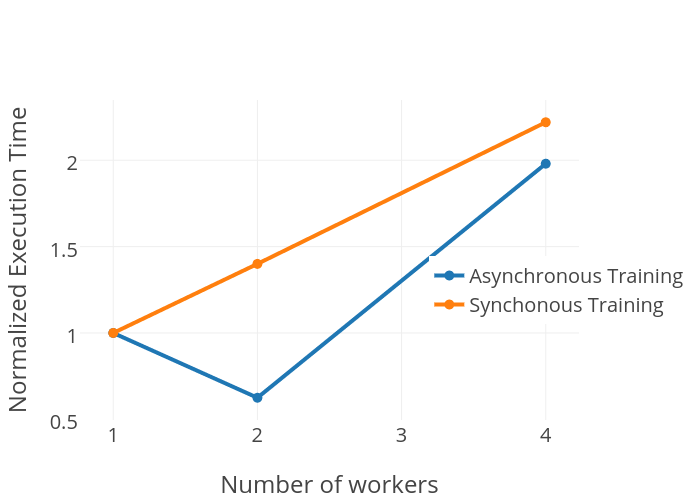
\includegraphics[keepaspectratio,width=.9\columnwidth]{figures/15712-corrected-scalability.png}
  \caption{\textbf{Scalability to multiple workers}}
  \label{fig:scalability}
\end{figure}

Figure \ref{fig:scalability} shows the execution time required 
to complete 20000 steps when run with 1,2 and 4 workers with
and without synchronization. The 
execution times for all the configurations are normalized to 
the single worker case. The data shows that the performance
of the precise and execution 





> Why distribute? 
Model parallelism allows training more complex models with many 
parameters. This is a progression from using GPUs to many different
machines. 

> synchronous training scalability. Impact of synchrony on accuracy
Why do we use synchronous training. Is it because we have a system
that is similar to the single node version? 
This berkeley thesis talks about why synchronization is important. 
Apparently synchronization allows for faster convergence because 
the average of the local updates of different machines reduces the
variance in data which leads to faster convergence. (https://www2.eecs.berkeley.edu/Pubs/TechRpts/2016/EECS-2016-47.pdf)
Blindly removing synchrony in an application does not seem to be
completely useful.

The impact of asynchrony on accuracy is that we are making judgements
on only part of the data that was present in our local store. This
higlights the dependence of the distribution of data and the homogeniety
(in terms of information) of the data. I think this was the premise of 
the hogwild paper.

> How does asynchrony affect training time? And accuracy
Stragglers are an issue in any large scale distributed training. If 
we use machines with different processing times (as in a distributed
cluster with different processing times) then the effects of stragglers
are exaggerated. 




